\clearpage
\newpage
\section{Specific Requirements}
\label{sec:reqs}
%include more details on all aspects of section 2 if they are useful for the development team

\subsection{External Interface Requirements}
\subsubsection{User Interfaces}
This section presents the user interfaces for the CodeKataBattles platform. The first section is dedicated to the user interfaces encountered by the student, and the second section to those encountered by the educator. While similar on many accounts as both students and educators need the ability to monitor and receive notifications about relevant tournaments and battles. However, students' interactions with battles and tournaments are limited to monitoring and subscribing, while educators can create new battles and tournaments. While the service needs to be accessed by a heterogeneous set of users, because a lot of the intricacies of the difference in use-cases are handled by GitHub, a lot of the functionalities available to students and educators are very closely related. 

\newpage
\clearpage
\subsection{Students}

\begin{figure}[Htbp!]
    \centering
    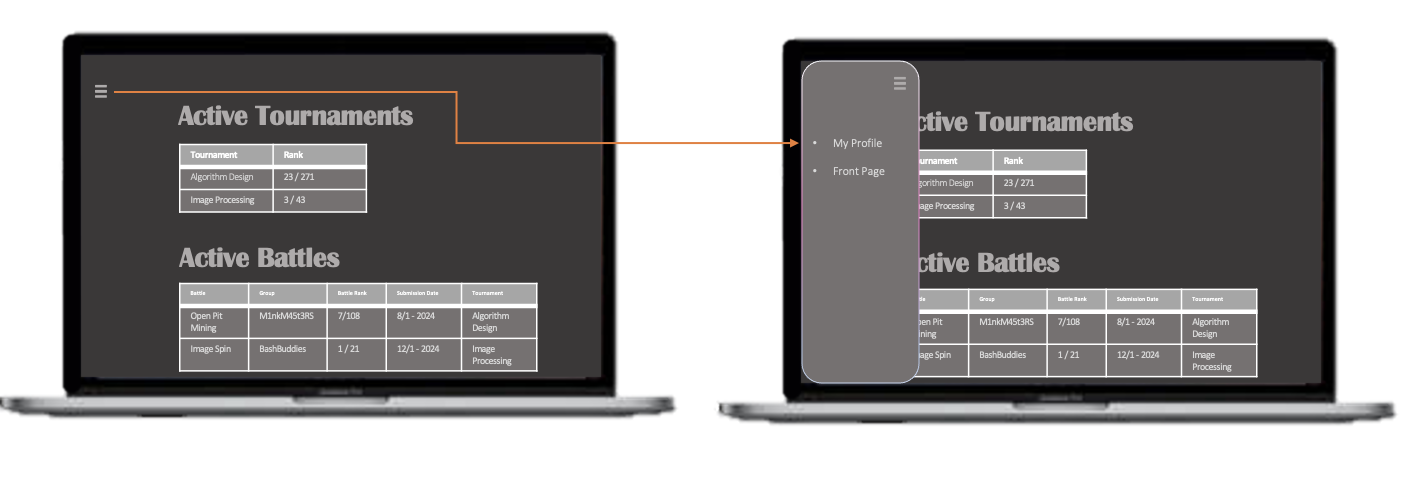
\includegraphics[width=\textwidth]{Graphics/SIDE BAR.png}
    \caption{User Interface: Front Page \& Sidebar}
    \label{fig:Sidebar}
\end{figure}

\begin{figure}[Htbp!]
    \centering
    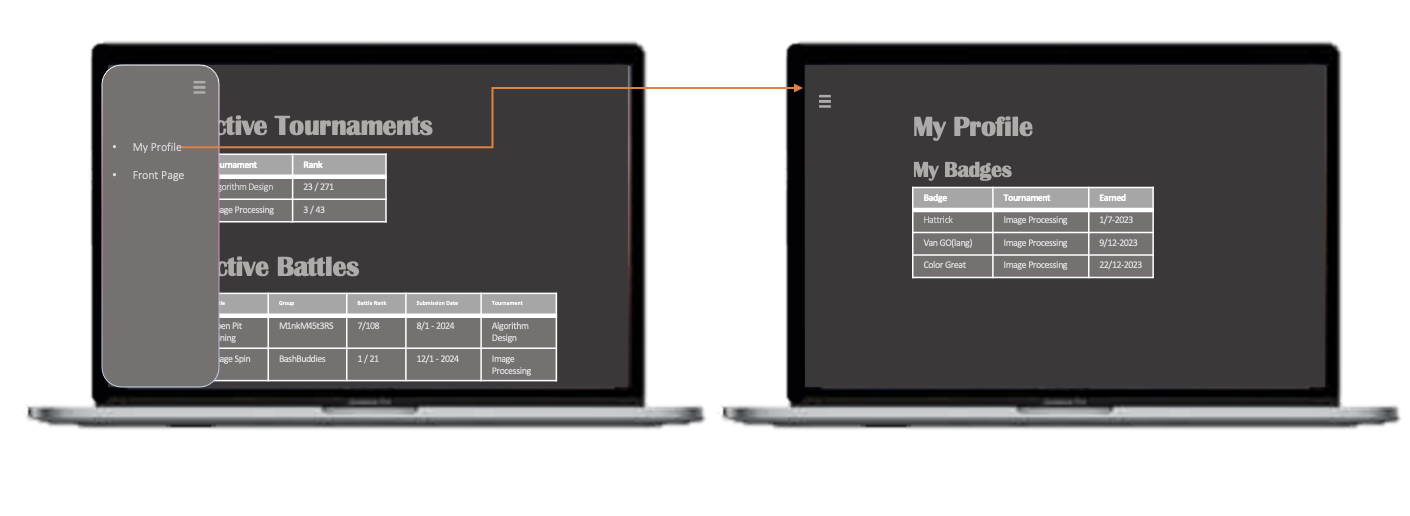
\includegraphics[width=\textwidth]{Graphics/MY PROFILE.png}
    \caption{User Interface: Profile}
    \label{fig:profile}
\end{figure}

\begin{figure}[Htbp!]
    \centering
    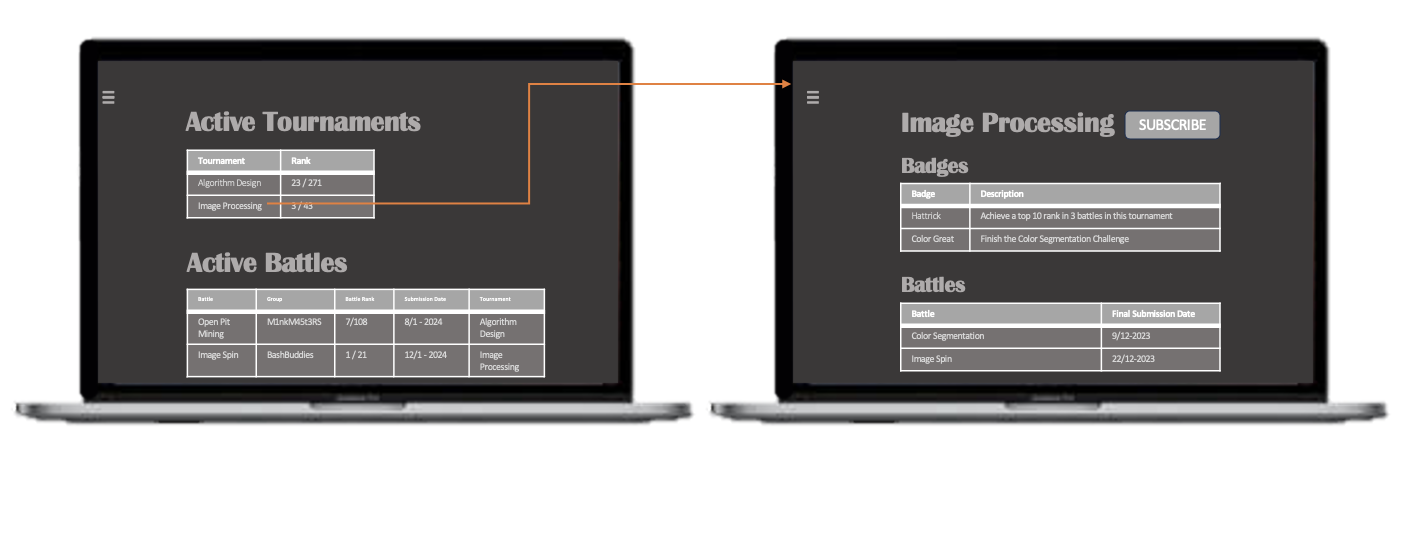
\includegraphics[width=\textwidth]{Graphics/TOURNAMENTS.png}
    \caption{User Interface: Tournament Page}
    \label{fig:tournaments}
\end{figure}


\begin{figure}[Htbp!]
    \centering
    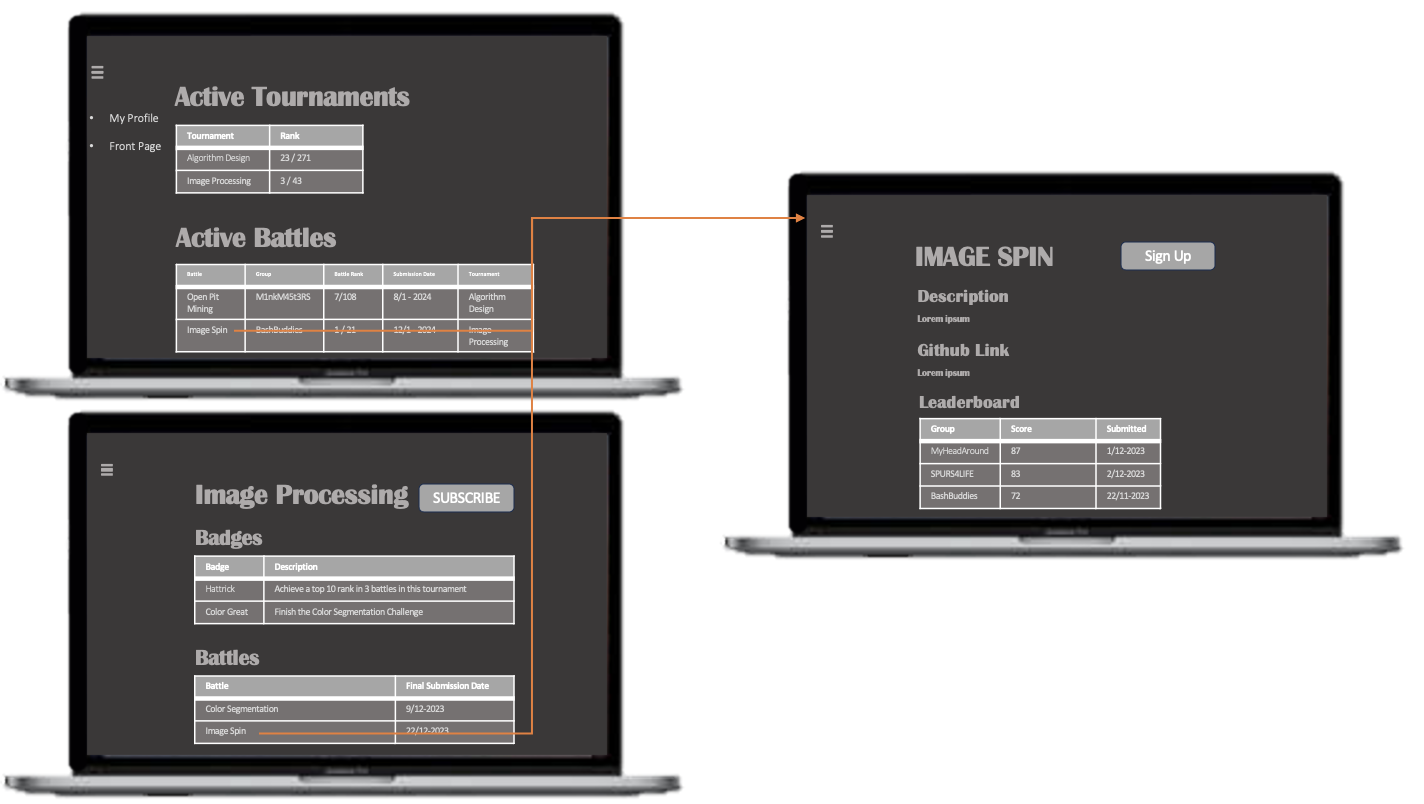
\includegraphics[width=\textwidth]{Graphics/BATTLE.png}
    \caption{User Interface: Battle Page}
    \label{fig:battle}
\end{figure}


\begin{figure}[Htbp!]
    \centering
    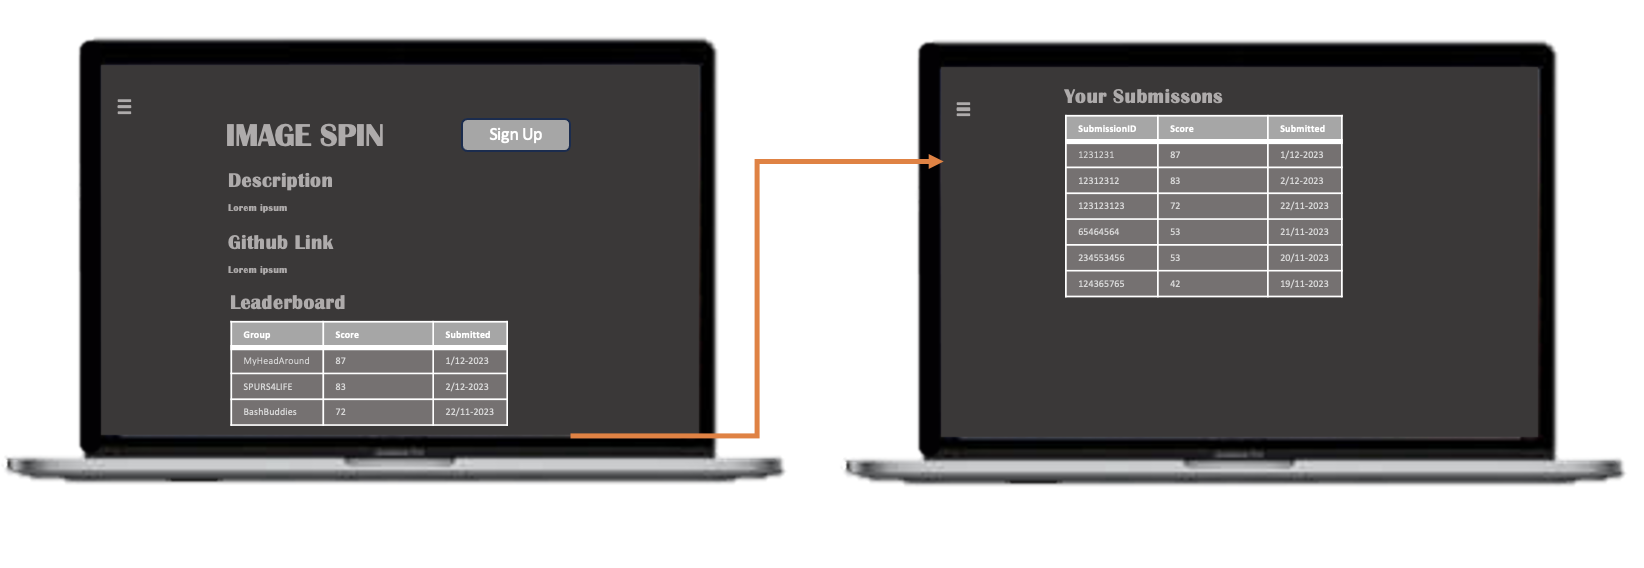
\includegraphics[width=\textwidth]{Graphics/SUBMISSION LOG.png}
    \caption{User Interface: Battle Page (Submission Log)}
    \label{fig:submissionlog}
\end{figure}

\subsection{Educators}

\begin{figure}[Htbp!]
    \centering
    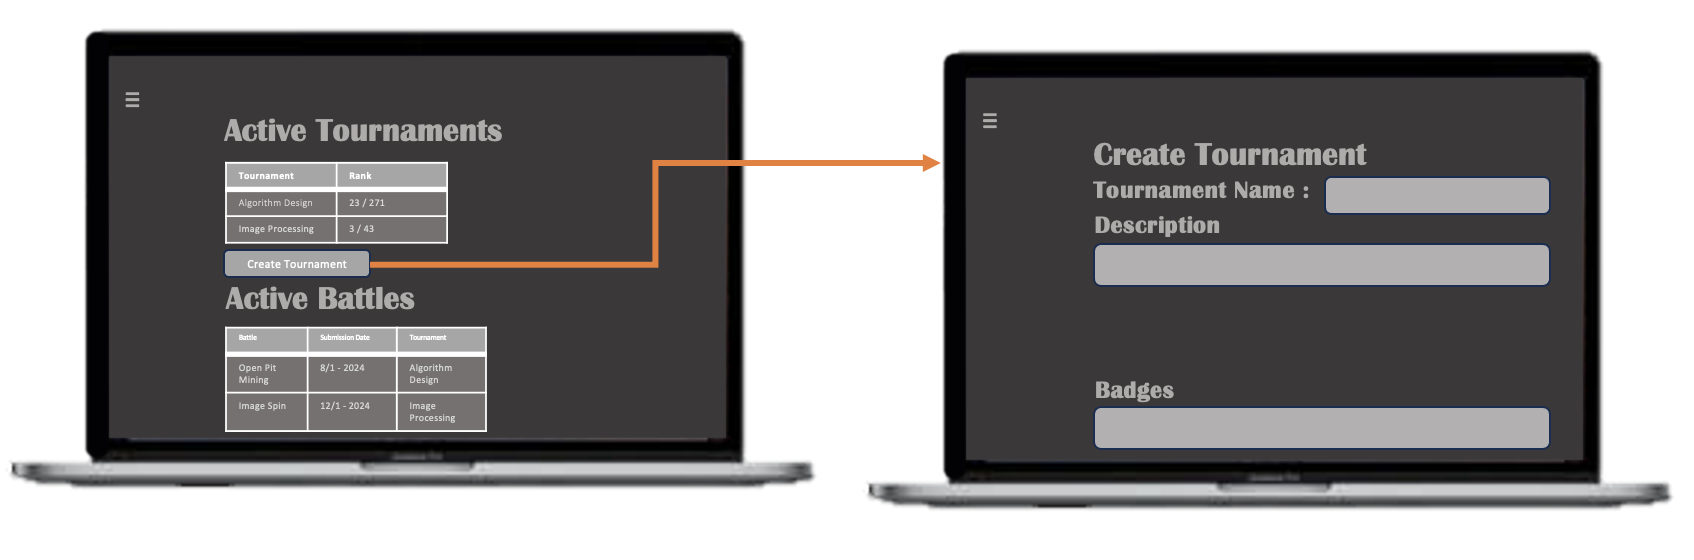
\includegraphics[width=\textwidth]{Graphics/CREATE TOURNAMENT.png}
    \caption{User Interface: Create Tournament Page}
    \label{fig:createTournament}
\end{figure}


\begin{figure}[Htbp!]
    \centering
    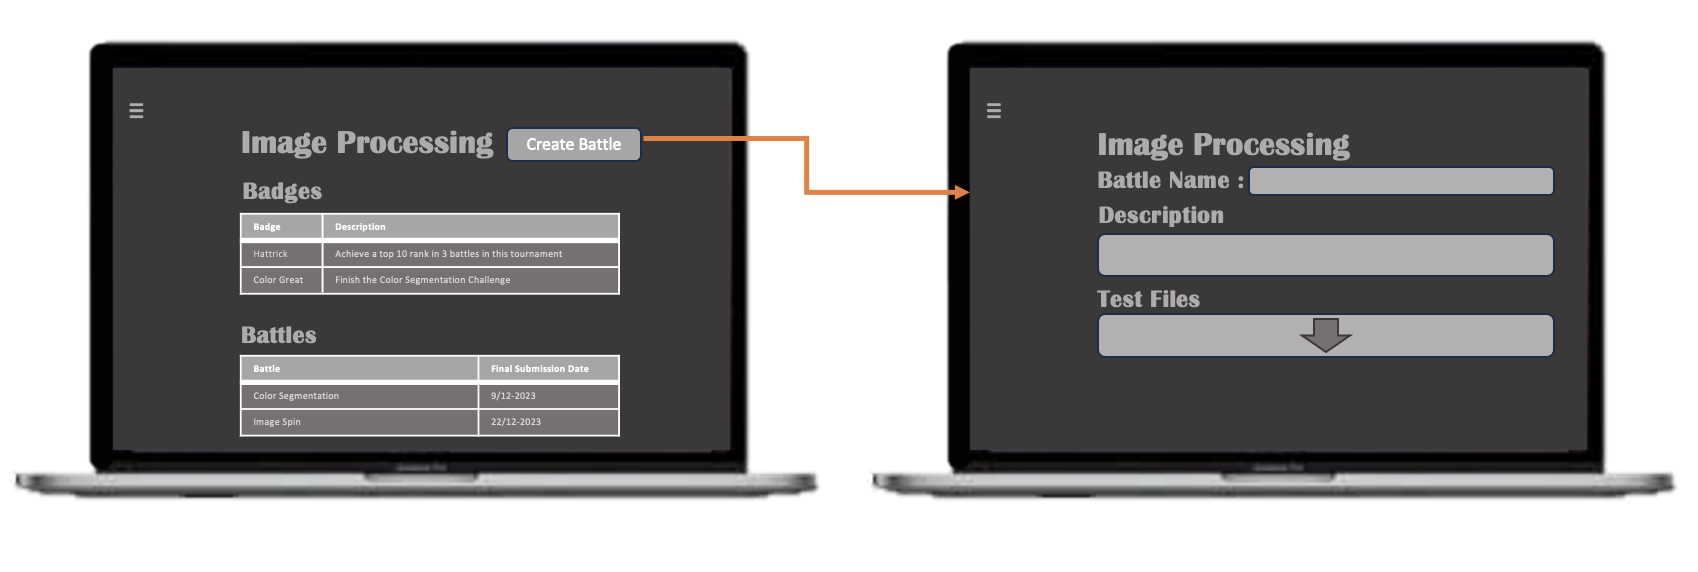
\includegraphics[width=\textwidth]{Graphics/CREATE BATTLE.png}
    \caption{User Interface: Create Battle Page}
    \label{fig:createBattle}
\end{figure}


\subsubsection{Hardware Interfaces}
All users, both Students and Educators can access the platform through a web browser. Therefore, all users need access to a device with an internet connection and browser installed. While note strictly required, a text editor is also recommended. 

\subsubsection{Software Interfaces}
The system utilizes one primary external service, namely Github. A Github action is set up, such that any pushes to a forked repository from a given battle is automatically pulled by the system. Then a predefined test script evaluates the implementation on a variety of tests.  

\subsection{Functional Requirements}
\label{sec:functional_requirements}

The CodeKataBattle system is designed to facilitate and manage competitive coding exercises, known as code katas. The system shall support the following functional requirements to ensure a comprehensive and engaging learning experience for students:

\begin{enumerate}
    \item \textbf{[R1]} The system shall allow users to sign up using their GitHub credentials (i.e. their email and GitHub Username).
    \item \textbf{[R2]} The system shall send a verification email to confirm a user's account upon sign-up.
    \item \textbf{[R3]} Educators shall be able to create tournaments with a specified title.
    \item \textbf{[R4]} Educators shall be able to set registration deadlines for tournaments.
    \item \textbf{[R5]} Educators shall be able to define tournament badge criteria.
    \item \textbf{[R6]} The system shall notify users of new tournaments.
    \item \textbf{[R7]} Users shall be able to subscribe to tournaments by a given deadline.
    \item \textbf{[R8]} Educators shall be able to create battles within tournaments.
    \item \textbf{[R9]} Educators shall be able to upload technical documents for battles.
    \item \textbf{[R10]} Educators shall be able to set the minimum and maximum number of students per group for battles.
    \item \textbf{[R11]} Educators shall be able to set a registration deadline for battles.
    \item \textbf{[R12]} Educators shall be able to set a final submission deadline for battles.
    \item \textbf{[R13]} Educators shall be able to configure scoring methodologies for battles.
    \item \textbf{[R14]} Students shall be able to form teams to join battles.
    \item \textbf{[R15]} The system shall provide a GitHub repository link for the code kata to registered teams after the registration deadline.
    \item \textbf{[R16]} The system shall automatically score submissions based on the results of test cases.
    \item \textbf{[R17]} The system shall evaluate the timeliness of submissions.
    \item \textbf{[R18]} The system shall assess the quality level of source code through static analysis.
    \item \textbf{[R19]} Educators shall have the option to manually score submissions.
    \item \textbf{[R20]} The system shall update battle scores in real-time upon new commits on GitHub.
    \item \textbf{[R21]} The system shall notify participants of final battle ranks after the consolidation phase.
    \item \textbf{[R22]} The system shall update personal tournament scores with the sum of battle scores.
    \item \textbf{[R23]} The system shall maintain a visible tournament rank for each student.
    \item \textbf{[R24]} Educators shall be able to define gamification badges with specific rules.
    \item \textbf{[R25]} The system shall display badges on student profiles.
    \item \textbf{[R26]} Educators shall be able to close tournaments and trigger final rank notifications.
    \item \textbf{[R27]} The system shall enable boolean expressions to define rules of badges and achievements.
    \item \textbf{[R28]} Students shall be able to visualize their performance.
    \item \textbf{[R29]} Students shall be able to visualize their tournament information.
    \item \textbf{[R30]} Students shall be able to track their battle involvement.
    \item \textbf{[R31]} Students shall be able to see detailed logs of their attempt outcomes.
\end{enumerate}

Definition of use case diagrams, use cases and associated sequence/activity diagrams, and mapping on requirements
 
\subsection{Performance Requirements}
\label{sec:performance_requirements}
The CodeKataBattles platform, recognizing the unique nature of code kata activities, has tailored performance requirements, especially concerning system downtime. Since a substantial part of the participation occurs in personal text editors or IDEs, the platform can accommodate longer downtimes without significantly impacting user productivity. An accepted downtime of up to half an hour is considered reasonable, allowing users to continue their work offline during such periods.

To minimize disruption, scheduled maintenance is planned during off-peak hours, and users are notified in advance through various channels. In case of unexpected downtimes, prompt communication is ensured, providing users with information and an estimated resolution time. Despite this tolerance for downtime, ensuring data integrity remains paramount. The platform is equipped with robust backup mechanisms to safeguard user data and maintain accessibility after downtimes.

These performance requirements reflect a balance between user experience and the practicalities of system maintenance for CodeKataBattles, catering to the platform's specific workflow.




\subsection{Design Constraints}

\subsubsection{Standards compliance}
Regarding data privacy, the CKB platform adheres to the General Data Protection Regulation (GDPR), which governs data protection and privacy for individuals within the European Union (EU) and the European Economic Area (EEA). Additionally, the system must comply with international standards for using and representing dates and times.

\subsubsection{Hardware limitations}
Here we report relevant hardware requirements. The only real hardware requirement is a machine with an Internet connection (2G/3G/4G/Wi-Fi) and a modern web browser

\subsection{Software System Attributes}
\subsubsection{Reliability}
As mentioned in section \ref{sec:performance_requirements} this service does not warrant complex infrastructure to aggressively reduce downtime, due to the amount of work being done in text editors or IDEs not directly connected to the platform. This is also the case for data, as all code is stored in Github repositories, however, all data related to the gamification aspect of the platform is stored only in the system. 

\subsubsection{Security}
As for any system handling personal information, such as CodeKataBattles does with information regarding educators and students, security is vital. 
To ensure compliance with security standards, encryption of passwords within the database must be applied. The same encryption need is present for data in transmission over the internet, to avoid interception-tactics. User's access to data must be a constraint to information deemed relevant for them through the use of role-based access control. 

\subsubsection{Availability}
CodeKataBattles is not a critical service, so the availability role is mainly to create a good user experience. Furthermore as mentioned in \ref{sec:performance_requirements} user productivity can exist in downtime. Therefore the system should aim to provide at least 99\% availability, meaning that the average time between occurrences of a failure and
service recovery (MTTR) must be less or equal to 3,65 days per year. 

\subsubsection{Maintainability}
The system is required to ensure a high level of maintainability. This entails the utilization of appropriate design patterns and adherence to recognized coding standards. The code must be well-documented, and practices such as hard-coding are strictly avoided. Moreover, the system should include a comprehensive testing routine, which is expected to cover a minimum of 75\% of the entire codebase, with the exception of interface code.

\subsubsection{Portability}
The web application should be compatible with all operating systems that support a web browser, including Windows, macOS, Linux, and others.

\begin{table}[h!]
\centering
\begin{tabular}{|p{0.2\textwidth}|p{0.7\textwidth}|}
\hline
\textbf{Name} & Login User \\
\hline
\textbf{Actors} & Student \& educator \\
\hline
\textbf{Entry Condition} & The student/educator has opened the CodeKata web application \\
\hline
\textbf{Event flow} & 
\begin{minipage}[t]{0.7\textwidth}
1 - The user inserts his username and password in the form \\
2 - The user clicks on the “Login” button \\
3 - The system checks the credentials \\
4 - The application shows the proper dashboard
\end{minipage} \\
\hline
\textbf{Exit condition} & The user has access to the services for the right interface provided by the CodeKata web application \\
\hline
\textbf{Exception} & 
\begin{minipage}[t]{0.7\textwidth}
3 - The data inserted are not valid. The system returns to the entry condition.
\end{minipage} \\
\hline
\end{tabular}
\caption{Use Case Specification}
\end{table}


\begin{table}[h!]
\centering
\begin{tabular}{|p{0.2\textwidth}|p{0.7\textwidth}|}
\hline
\textbf{Name} & Join tournament \\
\hline
\textbf{Actors} & Student \\
\hline
\textbf{Entry Condition} & 
\begin{minipage}[t]{0.7\textwidth}
1 - The student is logged into the CodeKata platform \\
2 - The student is on the home page of the CodeKata web application \\
3 - The registration deadline has not yet passed
\end{minipage} \\
\hline
\textbf{Event flow} & 
\begin{minipage}[t]{0.7\textwidth}
1 - The student selects one of the available tournaments on the homepage \\
2 - The student clicks on the “Join” button \\
3 - The system adds the specific user to the participant list for the given tournament \\
4 - The tournament is added to the overview of tournaments the student is currently participating in
\end{minipage} \\
\hline
\textbf{Exit condition} & 
The student now has access to the battles within the tournament and is returned to the tournament home page \\
\hline
\textbf{Exception} & \\
\hline
\end{tabular}
\caption{Use Case Specification}
\end{table}


\begin{table}[h!]
\centering
\begin{tabular}{|p{0.2\textwidth}|p{0.7\textwidth}|}
\hline
\textbf{Name} & Join battle \\
\hline
\textbf{Actors} & Student \\
\hline
\textbf{Entry Condition} & 
\begin{minipage}[t]{0.7\textwidth}
1 - The student is logged in \\
2 - The student is subscribed to the tournament, to which the battle belongs \\
3 - The battle is open for registration \\
4 - The student resides on the battles page
\end{minipage} \\
\hline
\textbf{Event flow} & 
\begin{minipage}[t]{0.7\textwidth}
1 - The student clicks on the “Join” button \\
2 - The student is prompted to specify participant(/s) by username in its group \\
3 - The student enters the name of the group \\
4 - The system adds the specific user/team to the participant list for the given battle \\
5 - The battle is added to the overview of battles the student is currently participating in
\end{minipage} \\
\hline
\textbf{Exit condition} & 
The student will now receive notifications relevant to the given battle and is returned to the battle's home page \\
\hline
\end{tabular}
\caption{Use Case Specification}
\end{table}




% Skal lige kigges over de her tables 
\begin{table}[h!]
\centering
\begin{tabular}{|l|l|}
\hline
\textbf{Name} & Create Battle \\
\hline
\textbf{Actors} & Educator \\
\hline
\textbf{Entry Condition} & 
\begin{tabular}[c]{@{}l@{}}
1 - The educator is logged into the CodeKata platform. \\
2 - The educator has the details of a specific tournament displayed. \\
\end{tabular} \\
\hline
\textbf{Event flow} & 
\begin{tabular}[c]{@{}l@{}}
1 - The educator clicks the “Create Battle” button. \\
2 - The educator uploads a brief textual description of the battle. \\
3 - The educator uploads a software project with build automation scripts. \\
4 - The educator sets the registration and submission deadlines. \\
5 - The educator selects the scoring methodology. \\
6 - The system confirms the creation of the battle. \\
\end{tabular} \\
\hline
\textbf{Exit condition} & 
The battle is created, enabling educator management within the tournament.\\
\hline
\textbf{Exception} & 
\begin{tabular}[c]{@{}l@{}}
If required details are missing or incorrect, the educator is prompted for correction. \\
\end{tabular} \\
\hline
\end{tabular}
\caption{Use Case Specification for Creating a Battle}
\end{table}

\begin{table}[h!]
\centering
\begin{tabular}{|l|l|}
\hline
\textbf{Name} & Manual Battle Evaluation \\
\hline
\textbf{Actors} & Educator \\
\hline
\textbf{Entry Condition} & 
\begin{tabular}[c]{@{}l@{}}
1 - The educator is logged in. \\
2 - The educator is the owner of the battle. \\
3 - The submission deadline for the battle has passed. \\
\end{tabular} \\
\hline
\textbf{Event flow} & 
\begin{tabular}[c]{@{}l@{}}
1 - The educator navigates to the battle's submission list. \\
2 - The educator selects a submission for review. \\
3 - The educator assesses the submission, assigning a manual score. \\
4 - The system updates the battle's rankings with the new score. \\
4 - The system notifies the creator/s of the submissions of evaluation. \\ %skal det her være en exit condition?
\end{tabular} \\
\hline
\textbf{Exit condition} & 
The evaluated submission has been scored and displayed in the battle's rankings. \\
\hline
\textbf{Exception} & 
\begin{tabular}[c]{@{}l@{}}
If an error occurs during scoring, the educator is notified to retry. \\
\end{tabular} \\
\hline
\end{tabular}
\caption{Use Case Specification for Evaluating a Submission}
\end{table}



\begin{table}[h!]
\centering
\begin{tabular}{|l|l|} 
\hline
\textbf{Name} & Create a Badge \\
\hline
\textbf{Actors} & Educator \\
\hline
\textbf{Entry Condition} & 
\begin{tabular}[c]{@{}l@{}}
1 - The educator is logged into the CodeKata platform. \\
2 - The educator is the creator of the tournament. \\
\end{tabular} \\
\hline
\textbf{Event flow} & 
\begin{tabular}[c]{@{}l@{}}
1 - The educator selects the option to create a new badge. \\
2 - The educator inputs the badge name, description, and criteria. \\
3 - The system validates the input and creates the badge. \\
\end{tabular} \\
\hline
\textbf{Exit condition} & 
A new badge is created and available for awarding to students in the tournament. \\
\hline
\textbf{Exception} & 
\begin{tabular}[c]{@{}l@{}}
If the criteria are not valid, the educator is prompted to correct the information. \\
\end{tabular} \\
\hline
\end{tabular}
\caption{Use Case Specification for Creating a Badge}
\end{table}

\begin{table}[h!]
\centering
\begin{tabular}{|l|l|}
\hline
\textbf{Name} & Check Tournament Ranking \\
\hline
\textbf{Actors} & Student \\
\hline
\textbf{Entry Condition} & 
\begin{tabular}[c]{@{}l@{}}
1 - The student is logged into the CodeKata platform. \\
2 - The student is participating in the tournament. \\
\end{tabular} \\
\hline
\textbf{Event flow} & 
\begin{tabular}[c]{@{}l@{}}
1 - The student navigates to the tournament overview. \\
2 - The student selects the tournament to view. \\
3 - The system displays the current ranking and score of all participants. \\
\end{tabular} \\
\hline
\textbf{Exit condition} & 
The student views their current standing within the tournament rankings. \\
\hline
\textbf{Exception} & 
\begin{tabular}[c]{@{}l@{}}
If the rankings are not available, the battle's start time is yet to be surpassed. \\
\end{tabular} \\
\hline
\end{tabular}
\caption{Use Case Specification for Checking Tournament Ranking}
\end{table}

\begin{table}[h!]
\centering
\begin{tabular}{|l|l|}
\hline
\textbf{Name} & Automatic Scoring of a Submission \\
\hline
\textbf{Actors} & System \\
\hline
\textbf{Entry Condition} & A group has submitted their solution. \\
\hline
\textbf{Event flow} & 
\begin{tabular}[c]{@{}l@{}}
1 - The system retrieves the latest commit from the group's GitHub repository. \\
2 - The system runs automated tests against the submission. \\
3 - The system calculates the score based on the test results. \\
4 - The system updates the battle's leaderboard with the new score. \\
\end{tabular} \\
\hline
\textbf{Exit condition} & 
The group's submission is scored and the leaderboard reflects the updated score. \\
\hline
\textbf{Exception} & 
\begin{tabular}[c]{@{}l@{}}
Errors during test execution or score calculation prompt system retry. \\
\end{tabular} \\
\hline
\end{tabular}
\caption{Use Case Specification for Automatic Scoring of a Submission}
\end{table}

\begin{table}[h!]
\centering
\begin{tabular}{|l|l|}
\hline
\textbf{Name} & Announcing Tournament Results \\
\hline
\textbf{Actors} & System \\
\hline
\textbf{Entry Condition} & 
\begin{tabular}[c]{@{}l@{}}
1 - All battles' submission deadlines within the tournament have passed.\\
2 - The tournament creator clicks the button on the tournament page to end it.  \\
\end{tabular} \\
\hline
\textbf{Event flow} & 
\begin{tabular}[c]{@{}l@{}}
1 - The system compiles final scores from all tournament battles. \\
2 - The system determines tournament winners and badge recipients. \\
3 - The system sends notifications to participants with final standings. \\
4 - The system updates the tournament page with the final results. \\
\end{tabular} \\
\hline
\textbf{Exit condition} & 
Participants get final results; standings are shown on the tournament page. \\
\hline
\textbf{Exception} & 
\begin{tabular}[c]{@{}l@{}}
Failure in result compilation or notification delivery triggers a retry. \\
\end{tabular} \\
\hline
\end{tabular}
\caption{Use Case Specification for Announcing Tournament Results}
\end{table}

\begin{table}[h!]
\centering
\begin{tabular}{|l|l|}
\hline
\textbf{Name} & View Tournament Ranking \\
\hline
\textbf{Actors} & Student, Educator \\
\hline
\textbf{Entry Condition} & 
The user is logged into the CodeKata platform and participating in a tournament. \\
\hline
\textbf{Event flow} & 
\begin{tabular}[c]{@{}l@{}}
1 - The user navigates to the specific tournament section. \\
2 - The user selects the option to view rankings. \\
3 - The system displays the leaderboard with student names and scores. \\
4 - User reviews the ranking positions and individual scores. \\
\end{tabular} \\
\hline
\textbf{Exit condition} & 
The user views their tournament ranking and scores. \\
\hline
\textbf{Exception} & 
\begin{tabular}[c]{@{}l@{}}
If the leaderboard isn't updated, the system suggests a page refresh. \\
\end{tabular} \\
\hline
\end{tabular}
\caption{Use Case Specification for Viewing Tournament Ranking}
\end{table}

\begin{table}[h!]
\centering
\begin{tabular}{|l|l|}
\hline
\textbf{Name} & Push a new commit to a battle solution\\
\hline
\textbf{Actors} & Student \\
\hline
\textbf{Entry Condition} & 
\begin{tabular}[c]{@{}l@{}}
1 - The student is logged into the CodeKata platform. \\
2 - The student is part of a group in an ongoing battle. \\
\end{tabular} \\
\hline
\textbf{Event flow} & 
\begin{tabular}[c]{@{}l@{}}
1 - The student updates their submission, by pushing a new commit in the forked GitHub repository. \\
2 - The system validates the submission and confirms receipt. \\
3 - The system queues the submission for scoring. \\
\end{tabular} \\
\hline
\textbf{Exit condition} & 
Submission is successfully uploaded and awaiting evaluation. Automatic submission evaluation is triggered. \\
\hline
\end{tabular}
\caption{Use Case Specification for Submitting a Solution}
\end{table}

\begin{table}[h!]
\centering
\begin{tabular}{|l|l|}
\hline
\textbf{Name} & Give out badges \\
\hline
\textbf{Actors} & System \\
\hline
\textbf{Entry Condition} & 
\begin{tabular}[c]{@{}l@{}}
1 - The educator in charge has closed the tournament. \\
2 - The final tournament rank became available. \\
\end{tabular} \\
\hline
\textbf{Event flow} & 
\begin{tabular}[c]{@{}l@{}}
1 - The badges associated to the turnament and the badges`s rules, which must be fulfilled to achieve the badge are checked. 2 - Each badge is assigned to one or more students. \\
\end{tabular} \\
\hline
\textbf{Exit condition} & 
Students involved in the tournament are notified of the final tournament rank and the awarded badges. \\
\hline
\end{tabular}
\caption{Use Case Specification for Submitting a Solution}
\end{table}

\begin{table}[h!]
\centering
\begin{tabular}{|l|l|}
\hline
\textbf{Name} & Create GitHub battle repository\\
\hline
\textbf{Actors} & System \\
\hline
\textbf{Entry Condition} & 
\begin{tabular}[c]{@{}l@{}}
1 - The registration deadline of a battle has expired. \\ \\
\end{tabular} \\
\hline
\textbf{Event flow} & 
\begin{tabular}[c]{@{}l@{}}
1 - The system creates a GitHub repository for the battle, containing the kata code. \\
\end{tabular} \\
\hline
\textbf{Exit condition} & 
Students of teams subscribed to the battle are being sent the link to the repository. \\
\hline
\end{tabular}
\caption{Use Case Specification for Submitting a Solution}
\end{table}

\begin{table}[h!]
\centering
\begin{tabular}{|l|l|}
\hline
\textbf{Name} & Finalise team battle score \\
\hline
\textbf{Actors} & System \\
\hline
\textbf{Entry Condition} & 
\begin{tabular}[c]{@{}l@{}}
1 - The submission deadline of the battle has expired \\
2 - Both mandatory automatic as well as optional manual evaluation have been completed. \\
\end{tabular} \\
\hline
\textbf{Event flow} & 
\begin{tabular}[c]{@{}l@{}}
1 - The teams final score of the battle is determined \\
\end{tabular} \\
\hline
\textbf{Exit condition} & 
1 - The teams members` tournament score is updated based on their achieved final battle score. \\
\hline
\end{tabular}
\caption{Use Case Specification for Submitting a Solution}
\end{table}

\begin{figure}[Htp]
\centering
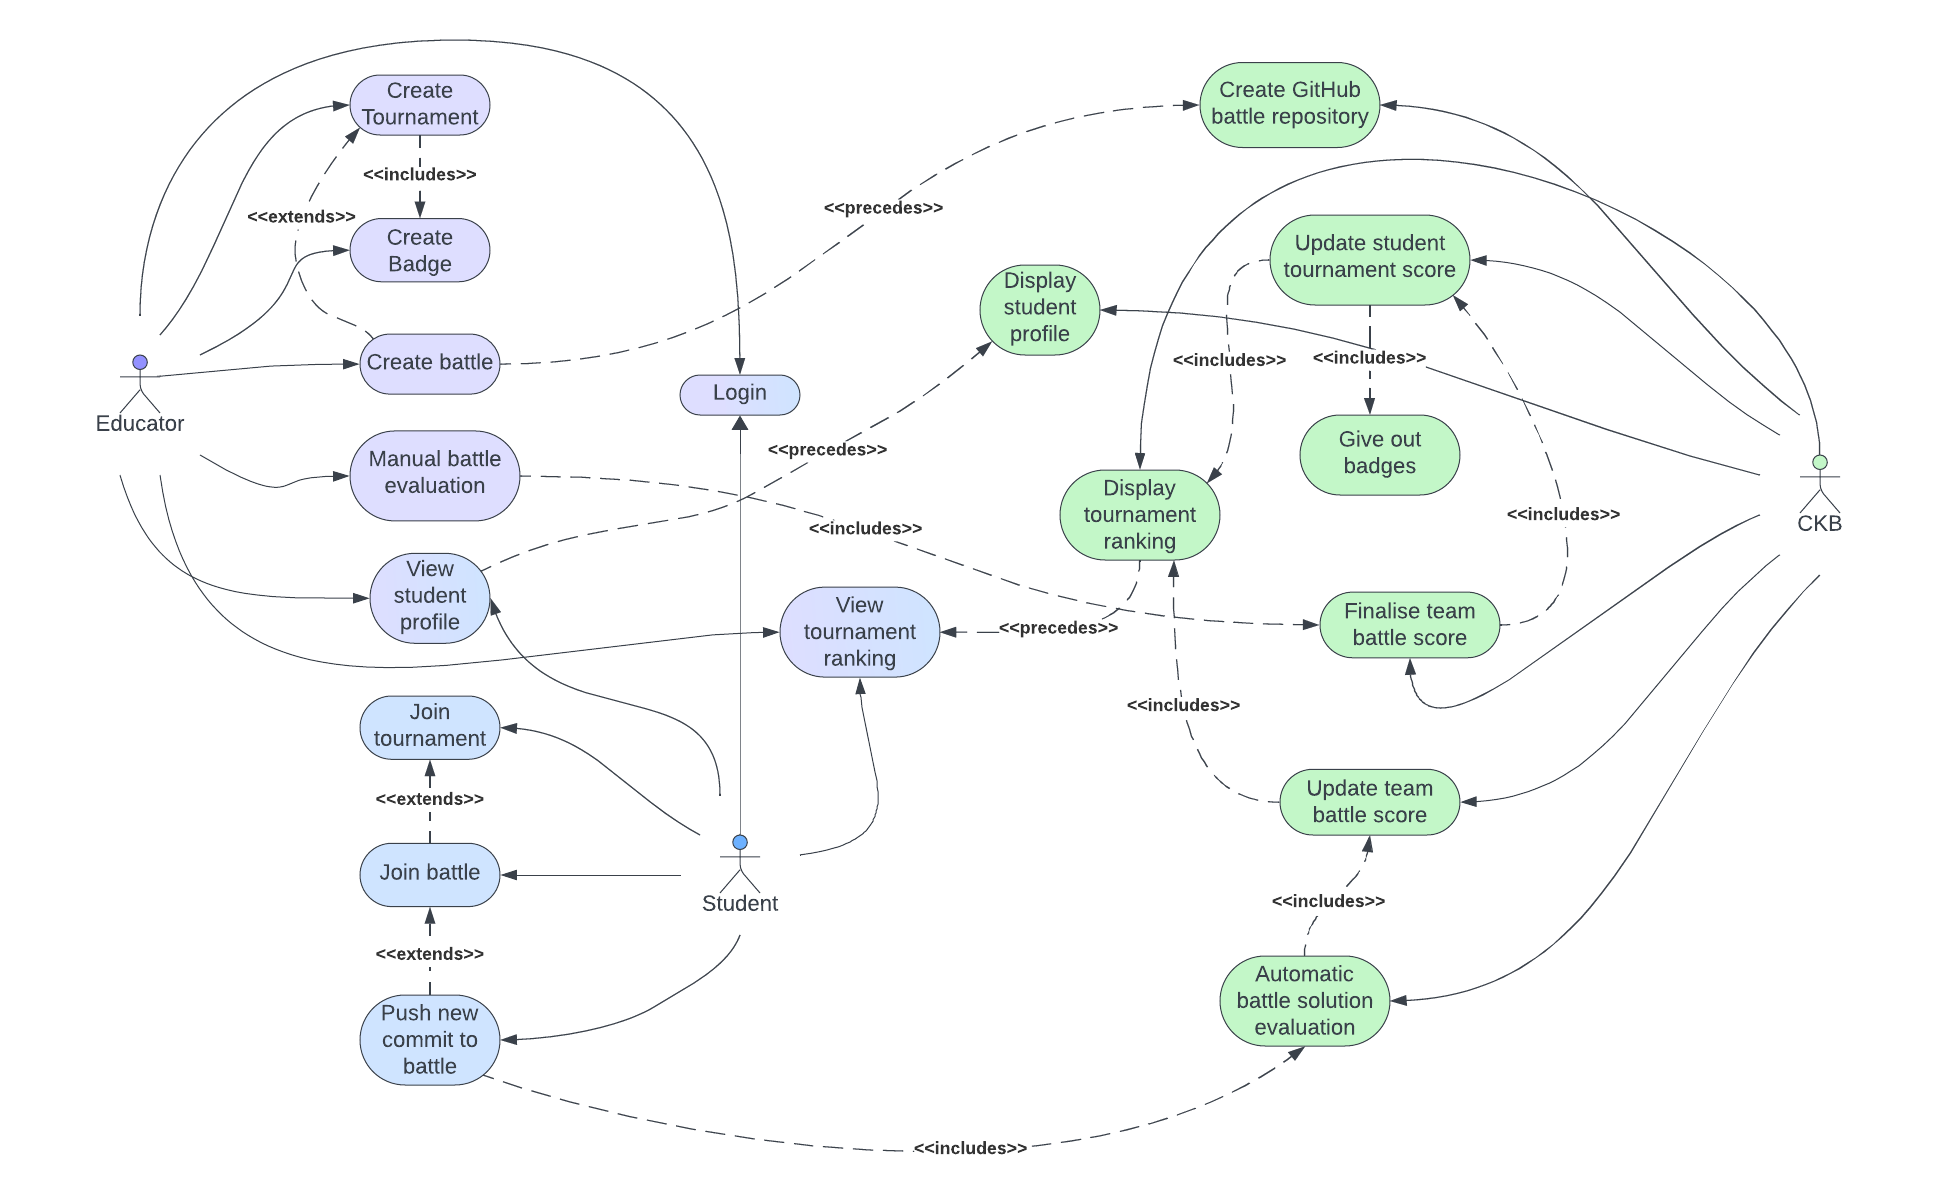
\includegraphics[width=\textwidth]{Graphics/Use case diagram.png}
\caption{Use case diagram.}
\label{fig:use case diagram}
\end{figure}

\clearpage
\newpage





\subsection{Requirements Mapping}
\label{sec:requirements_mapping}

This section maps the functional requirements and domain assumptions to the specific goals of the CodeKataBattle project. This mapping ensures that each goal is achievable through the fulfillment of certain requirements under the given assumptions.

\subsection{Goals to Requirements and Domain Assumptions}


% Goal 1
\begin{longtable}{|p{0.5\textwidth}|p{0.5\textwidth}|}
\hline
\multicolumn{2}{|c|}{\begin{minipage}{0.9\textwidth}
\centering
\vspace{5pt}
\textbf{[G2] Enable Educators to set up test-driven coding challenges including automated feedback online}
\vspace{5pt}
\end{minipage}} \\
\hline
\textbf{Requirements} & \textbf{Domain Assumptions} \\
\hline
R3-R5 Tournament creation with badges & D4 Educators' understanding of version control \\
R8-R13 Battle setup with technical documents and deadlines & D5 Correct automated testing scripts \\
R19 Manual scoring option for educators & R27 Boolean expressions for badge rules \\
\hline
\end{longtable}

% Goal 2
\begin{longtable}{|p{0.5\textwidth}|p{0.5\textwidth}|}
\hline
\multicolumn{2}{|c|}{\begin{minipage}{0.9\textwidth}
\centering
\vspace{5pt}
\textbf{[G2] Enable Educators to set up test-driven coding challenges including automated feedback online}
\vspace{5pt}
\end{minipage}} \\
\hline
\textbf{Requirements} & \textbf{Domain Assumptions} \\
\hline
R3-R5 Tournament creation with badges & D4 Educators' understanding of version control \\
R8-R13 Battle setup with technical documents and deadlines & D5 Correct automated testing scripts \\
R19 Manual scoring option for educators & R27 Boolean expressions for badge rules \\
\hline
\end{longtable}


% Goal 3
\begin{longtable}{|p{0.5\textwidth}|p{0.5\textwidth}|}
\hline
\multicolumn{2}{|c|}{\begin{minipage}{0.9\textwidth}
\centering
\vspace{5pt}
\textbf{[G3] Simulate a Real-world software development scenario through the use of GitHub and GitHub Actions.}
\vspace{5pt}
\end{minipage}} \\
\hline
\textbf{Requirements} & \textbf{Domain Assumptions} \\
\hline
R15 Use of GitHub repositories for code katas & D10 Compatibility with code kata requirements \\
R17 Timeliness evaluation of submissions & D13 Adherence to test-first development approach \\
\hline
\end{longtable}

% Goal 4
\begin{longtable}{|p{0.5\textwidth}|p{0.5\textwidth}|}
\hline
\multicolumn{2}{|c|}{\begin{minipage}{0.9\textwidth}
\centering
\vspace{5pt}
\textbf{[G4] Enable Educators to set up test-driven coding challenges including automated feedback online}
\vspace{5pt}
\end{minipage}} \\
\hline
\textbf{Requirements} & \textbf{Domain Assumptions} \\
\hline
R22 Update of personal tournament scores & D14 Use of scores for constructive feedback \\
R23 Maintenance of visible tournament rank & D15 Fair use of the platform by users \\
R28-R30 Performance visualization tools &  \\
\hline
\end{longtable}

\subsection{Sequence Diagrams}

\begin{figure}[Htbp!]
    \centering
    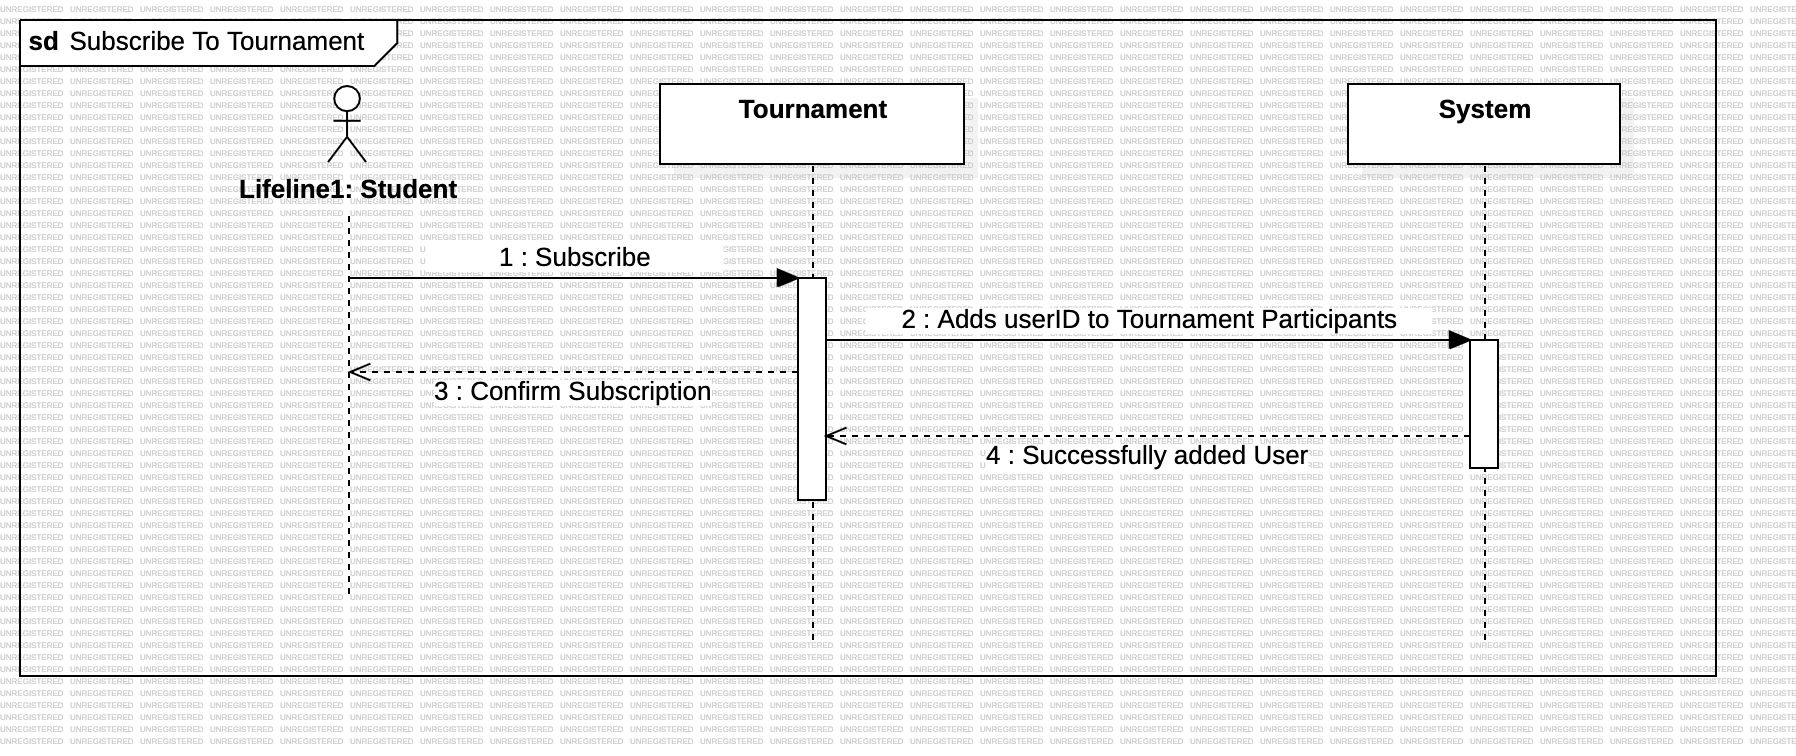
\includegraphics[width=\textwidth]{Graphics/Sequence Diagrams/SubscribeToTournament.png}
    \caption{Sequence Diagram: Subscribe to Tournament}
    \label{fig:Subscribe}
\end{figure}


\begin{figure}[Htbp!]
    \centering
    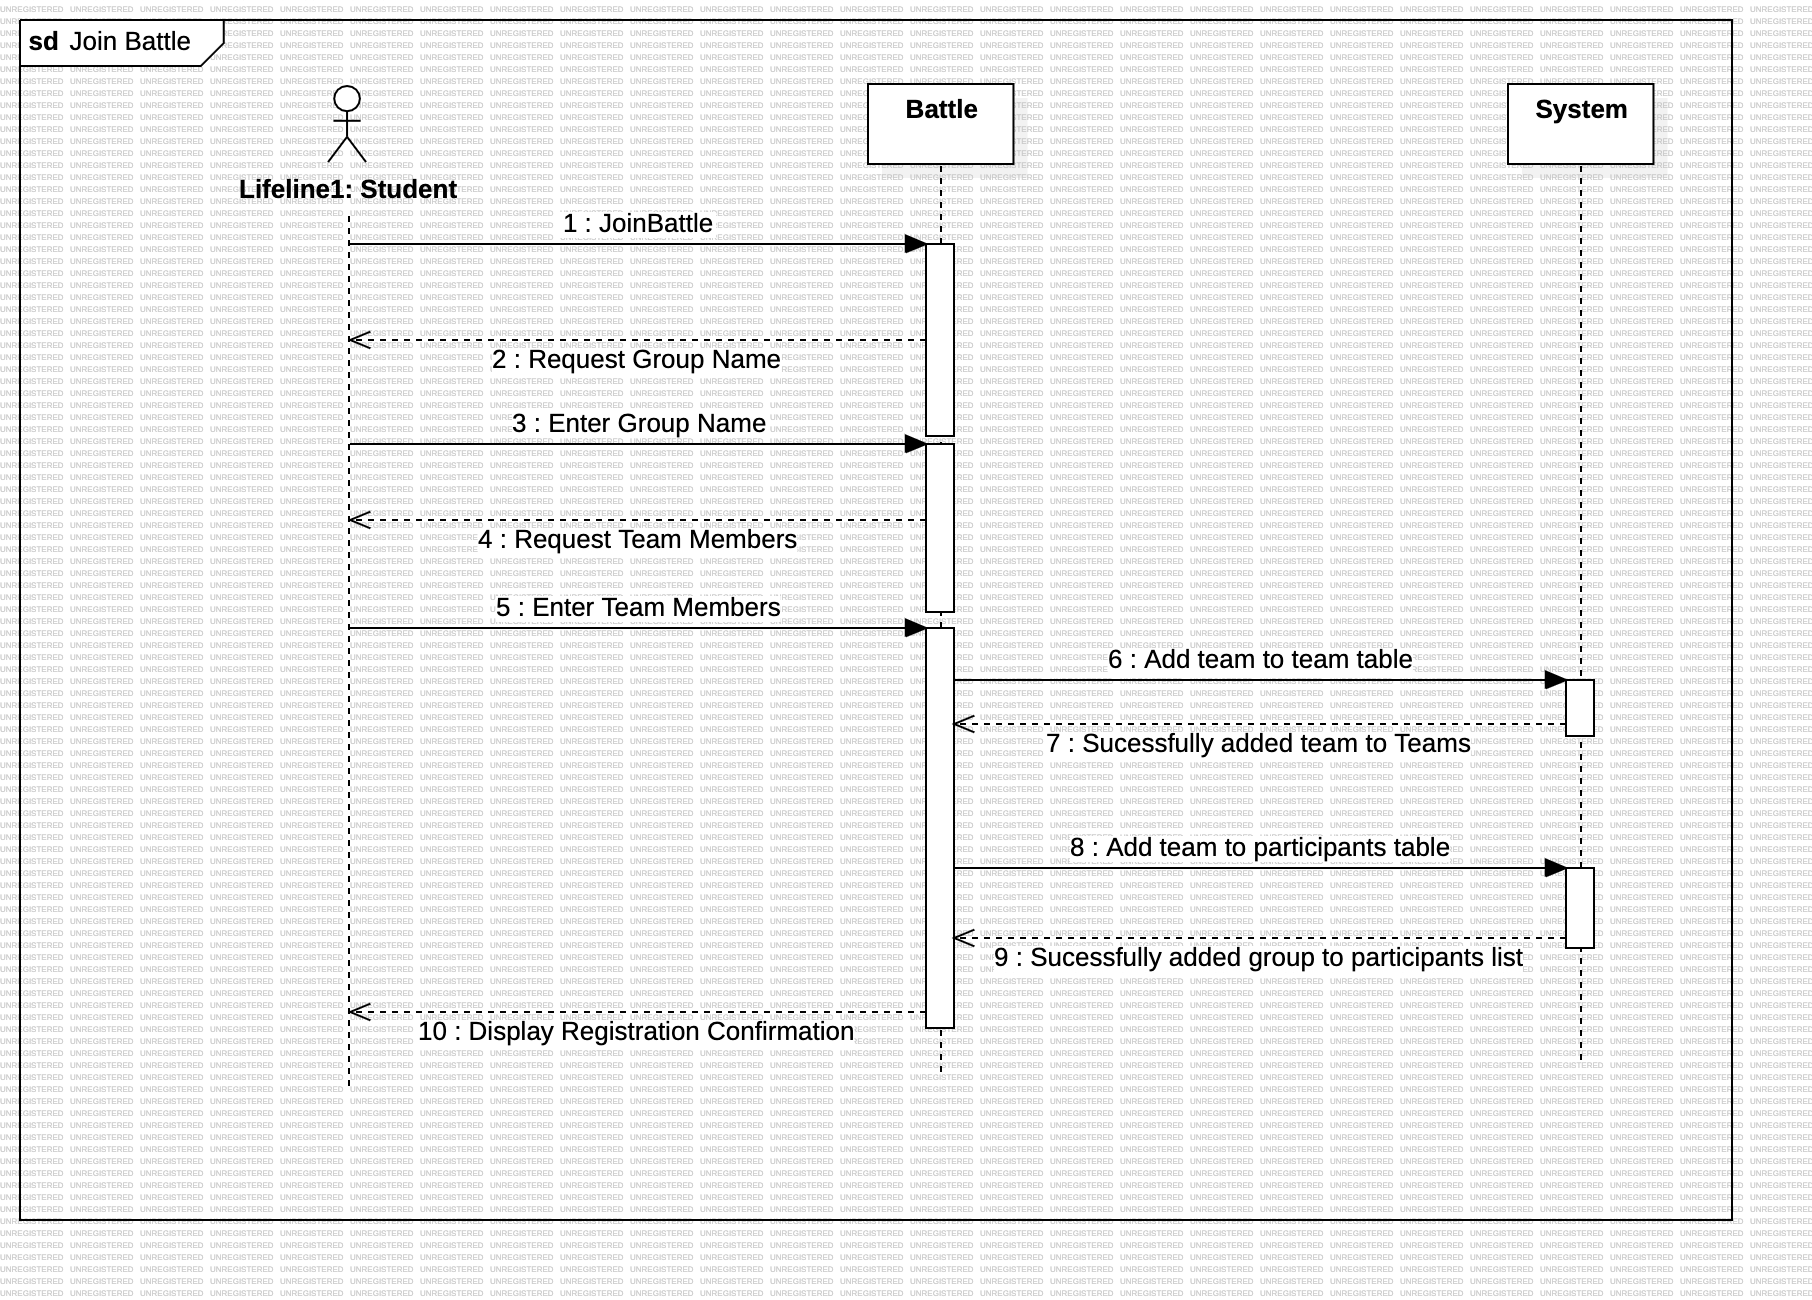
\includegraphics[width=\textwidth]{Graphics/Sequence Diagrams/Join Battle.png}
    \caption{Sequence Diagram: Join Battle}
    \label{fig:Join}
\end{figure}

\newpage

\begin{figure}[Htbp!]
    \centering
    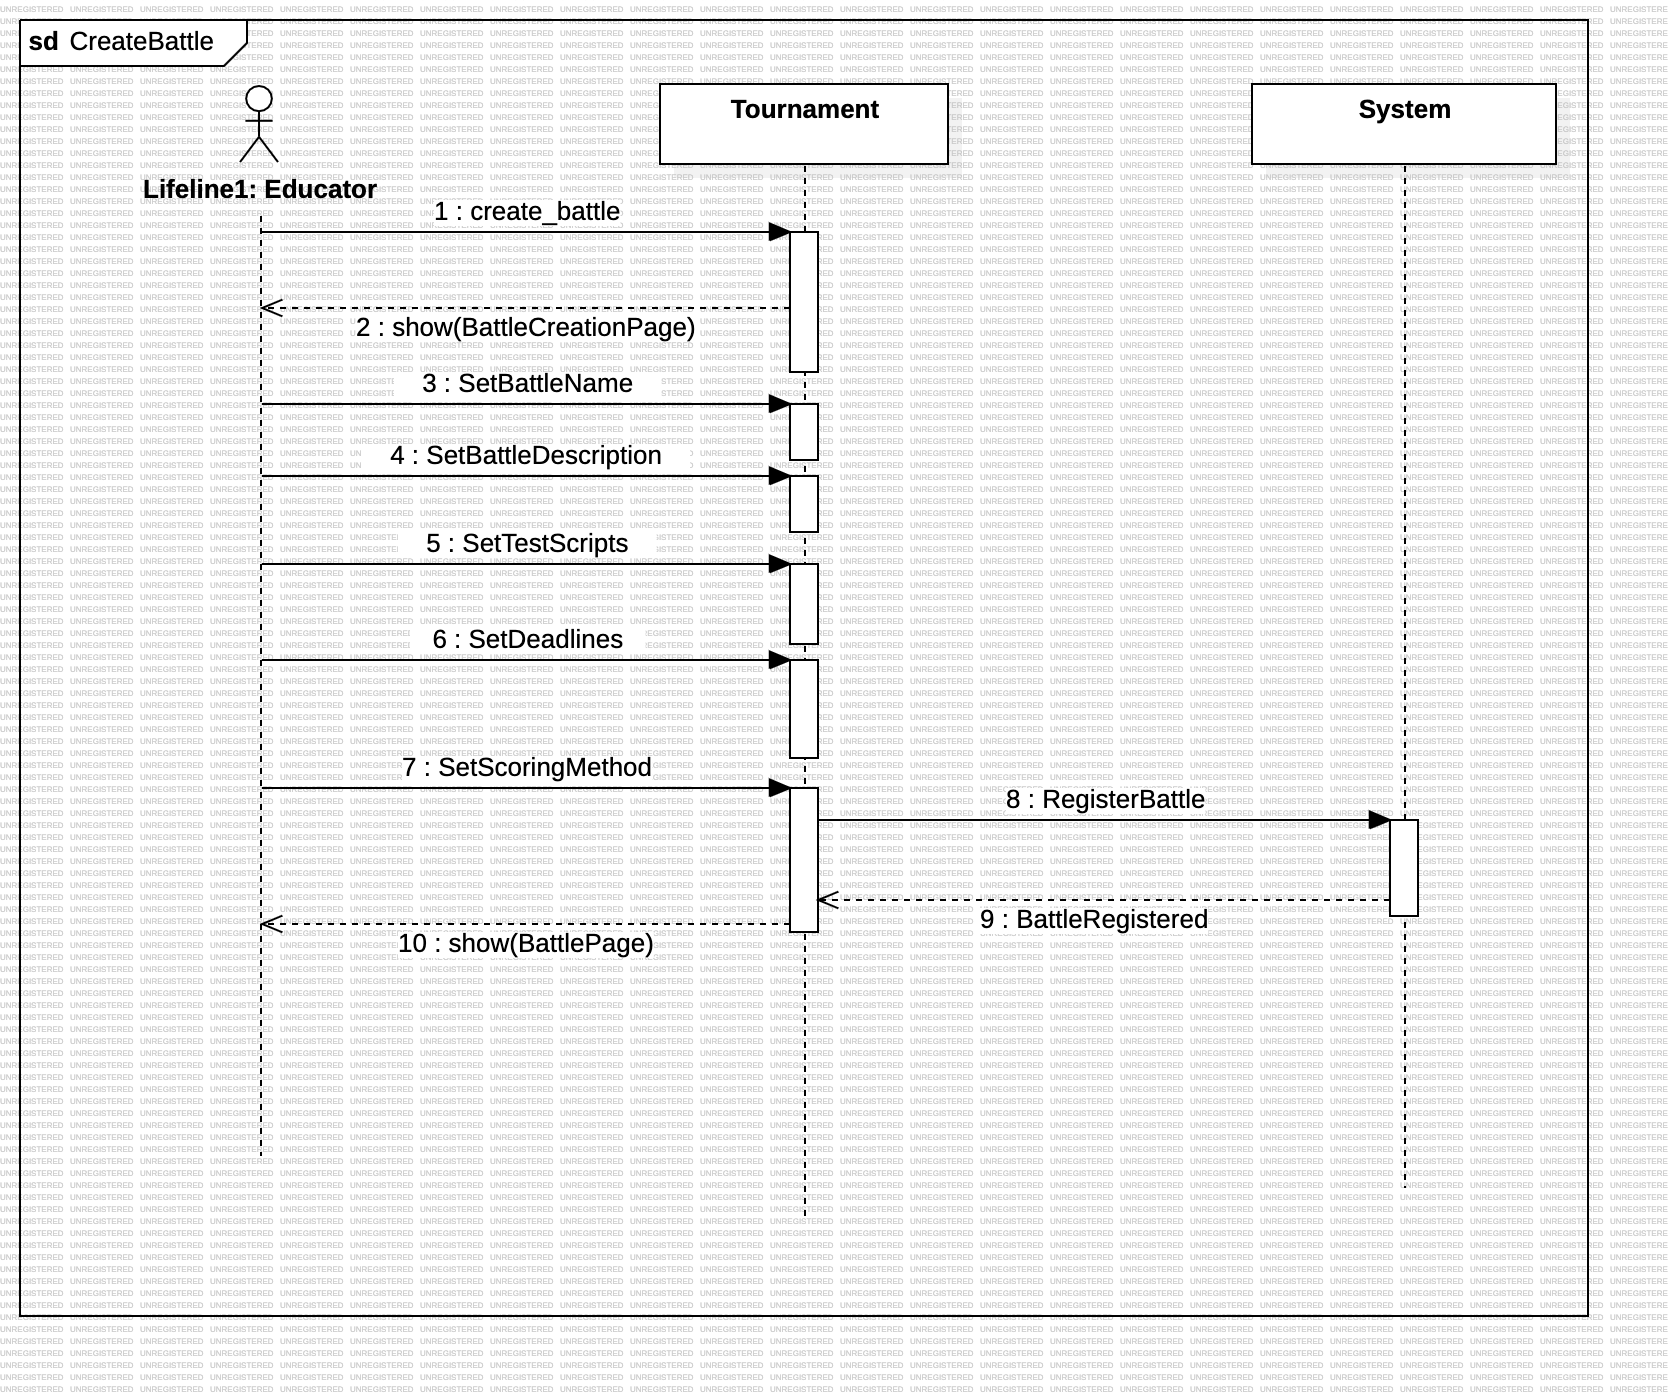
\includegraphics[width=\textwidth]{Graphics/Sequence Diagrams/CreateBattle.png}
    \caption{Sequence Diagram: Create Battle}
    \label{fig:CreateBattle}
\end{figure}



\begin{figure}[Htbp!]
    \centering
    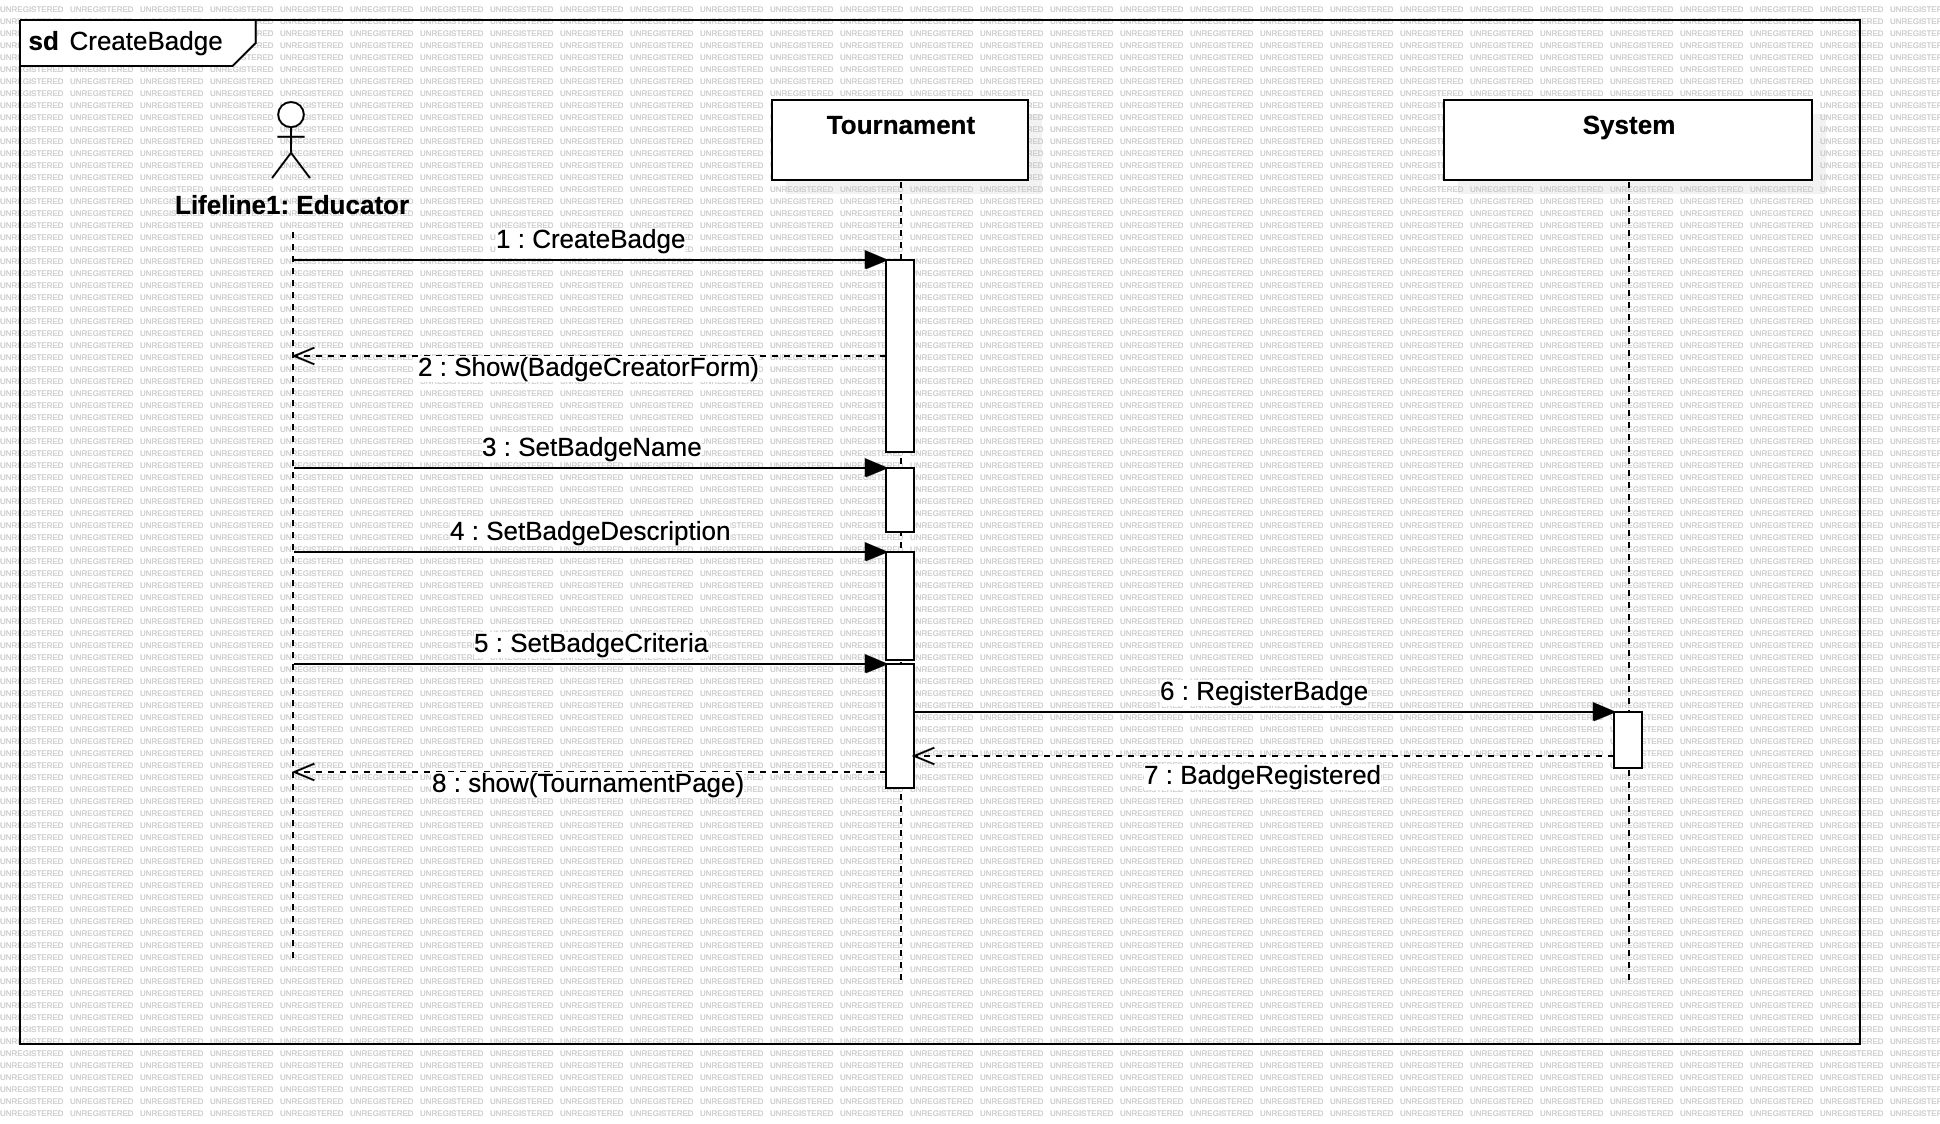
\includegraphics[width=\textwidth]{Graphics/Sequence Diagrams/CreateBadge.png}
    \caption{Sequence Diagram: Create Badge}
    \label{fig:CreateBadge}
\end{figure}
\newpage

\begin{figure}[Htbp!]
    \centering
    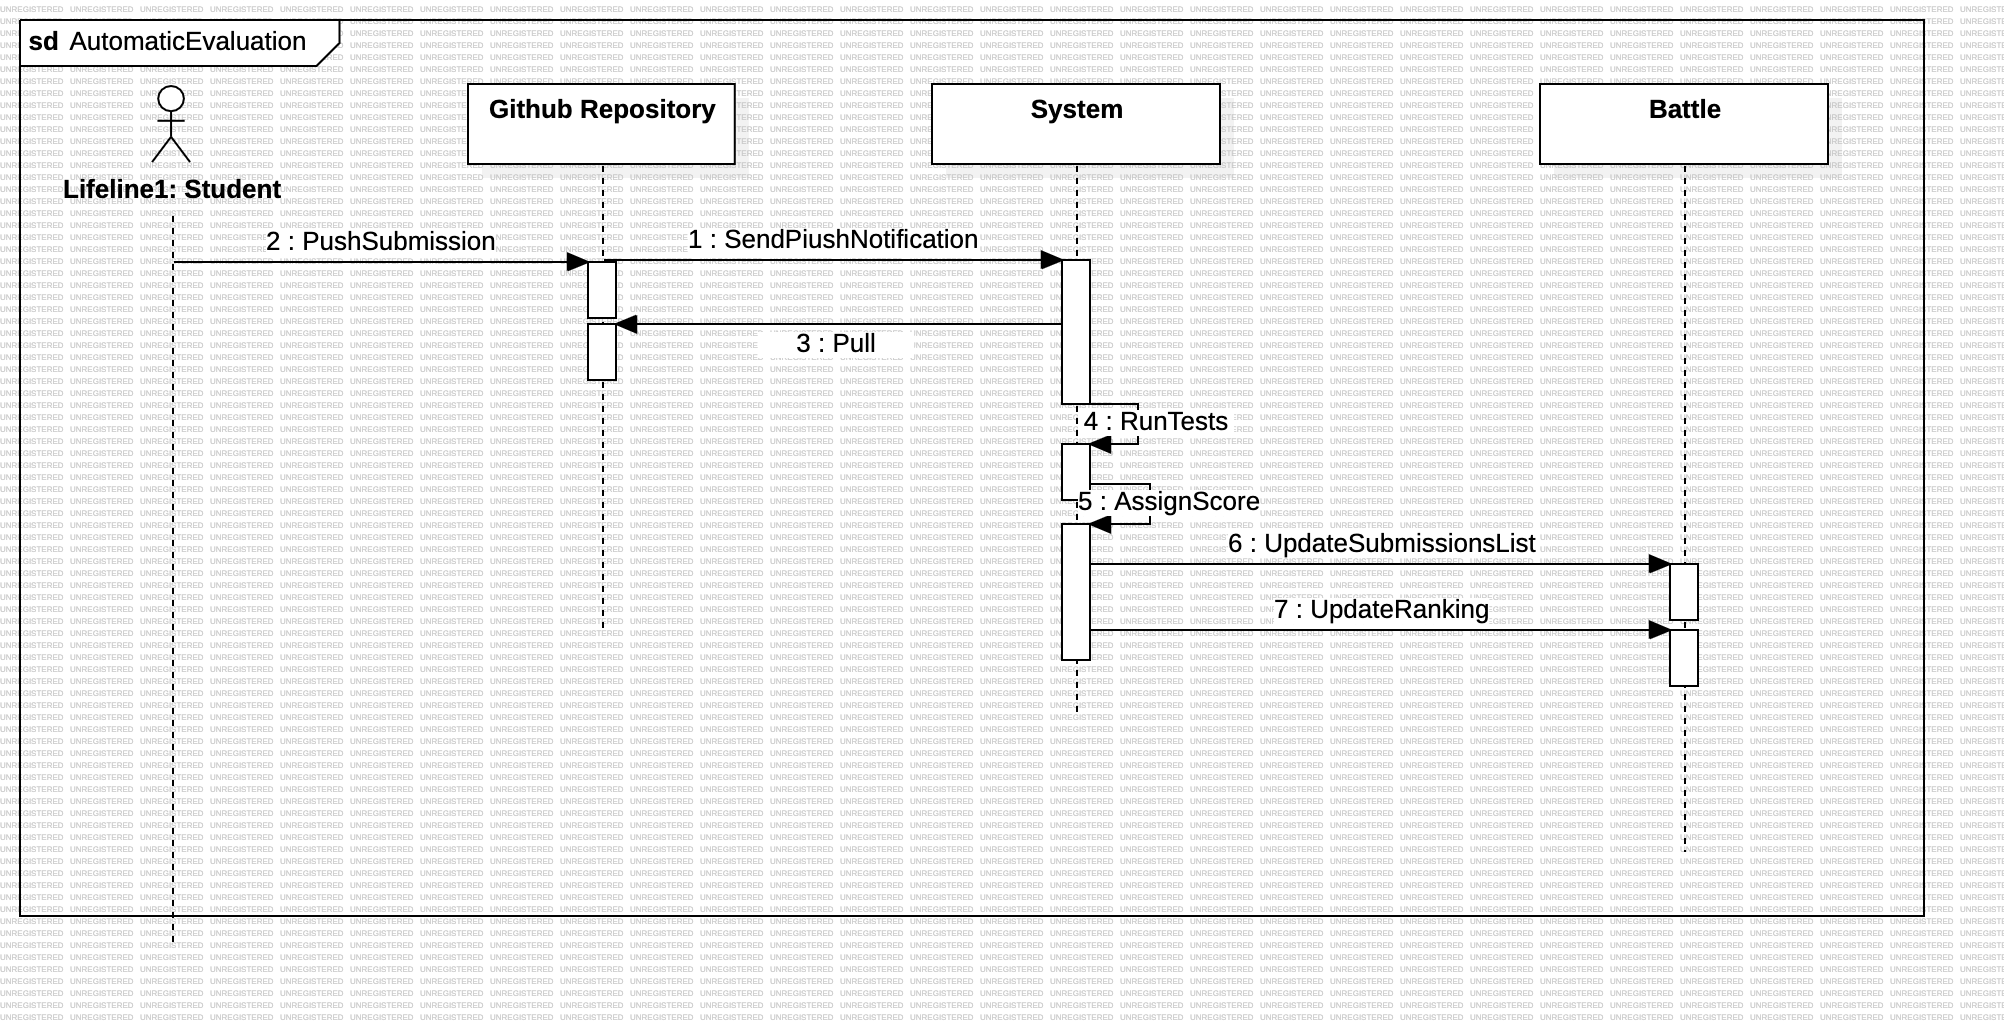
\includegraphics[width=\textwidth]{Graphics/Sequence Diagrams/AutomaticEvaluation.png}
    \caption{Sequence Diagram: Automatic Evaluation}
    \label{fig:AutoEval}
\end{figure}


\begin{figure}[Htbp!]
    \centering
    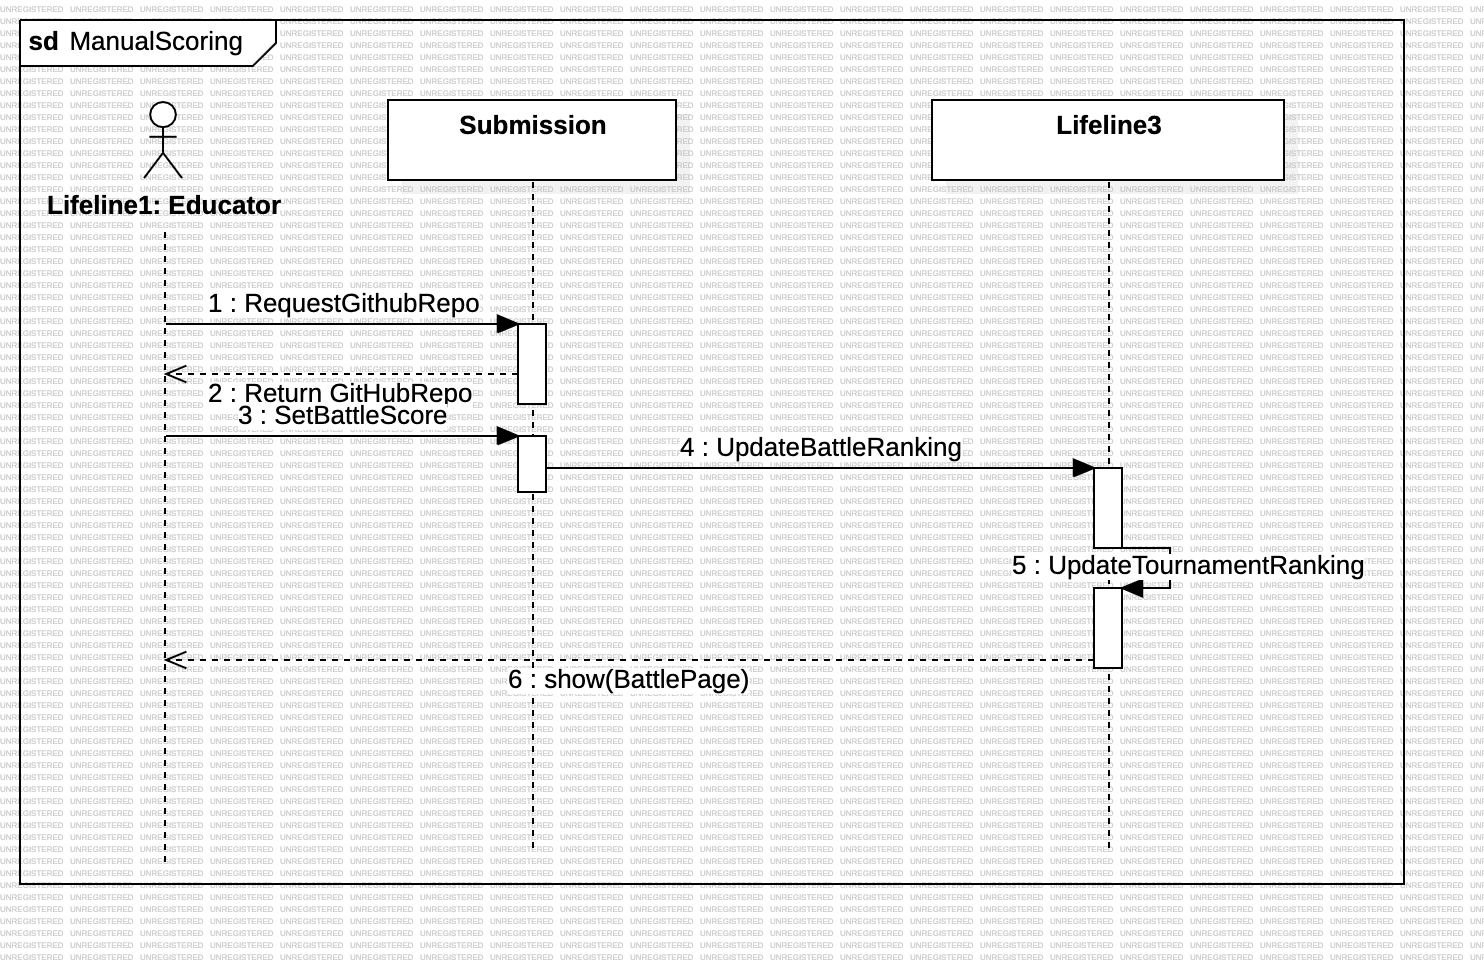
\includegraphics[width=\textwidth]{Graphics/Sequence Diagrams/ManualScoring.png}
    \caption{Sequence Diagram: Manual Evaluation }
    \label{fig:ManEval}
\end{figure}

\newpage
\begin{figure}[Htbp!]
    \centering
    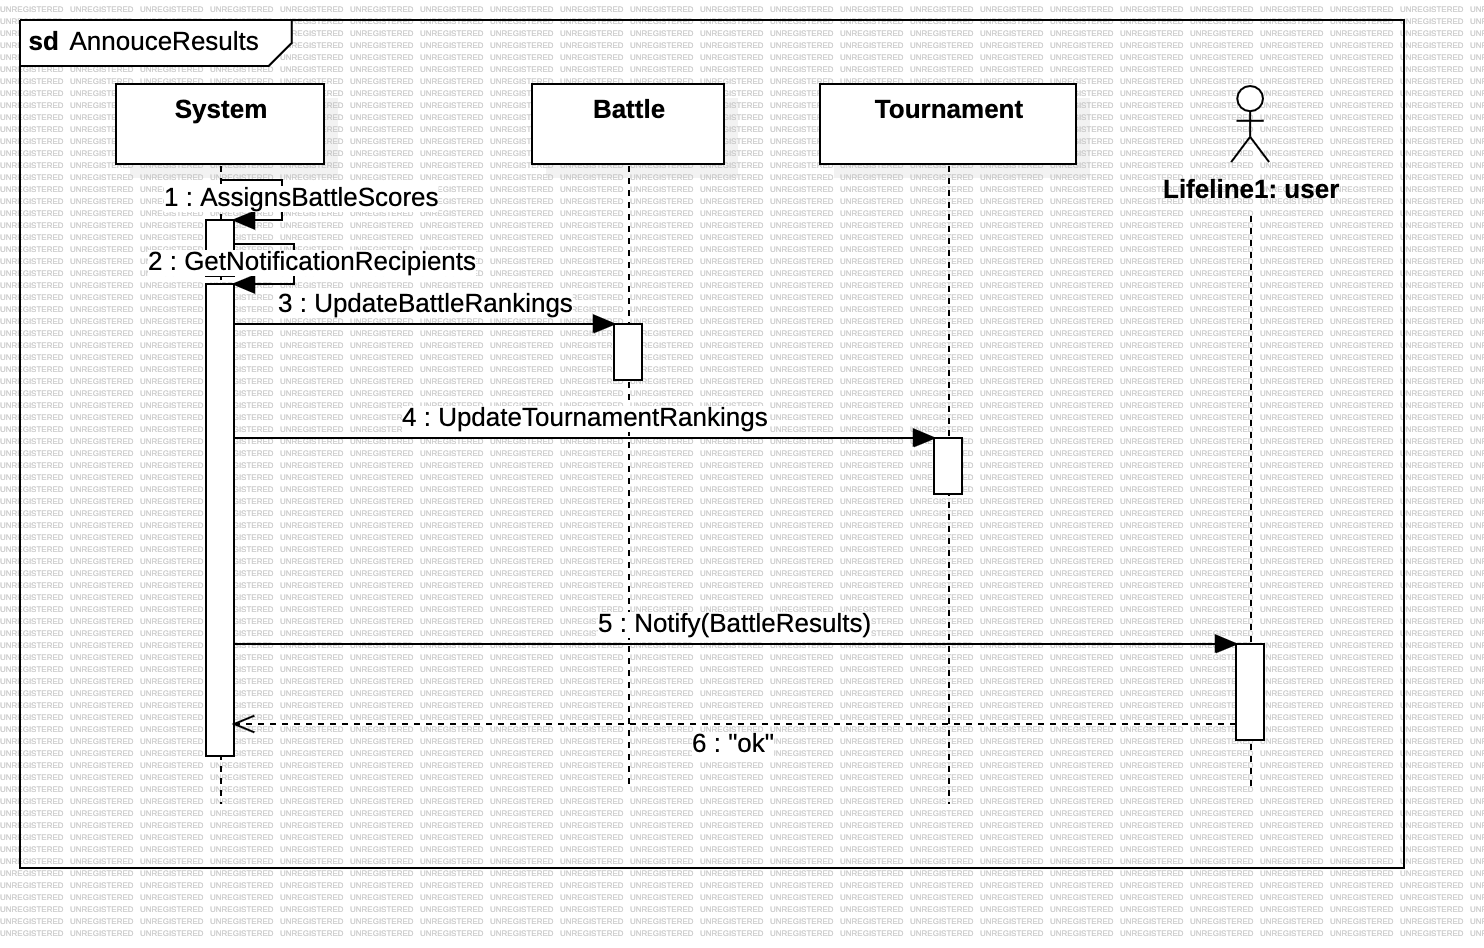
\includegraphics[width=\textwidth]{Graphics/Sequence Diagrams/AnnouceResults.png}
    \caption{Sequence Diagram: Announce Battle Results}
    \label{fig:Announcement}
\end{figure}



\begin{figure}[Htbp!]
    \centering
    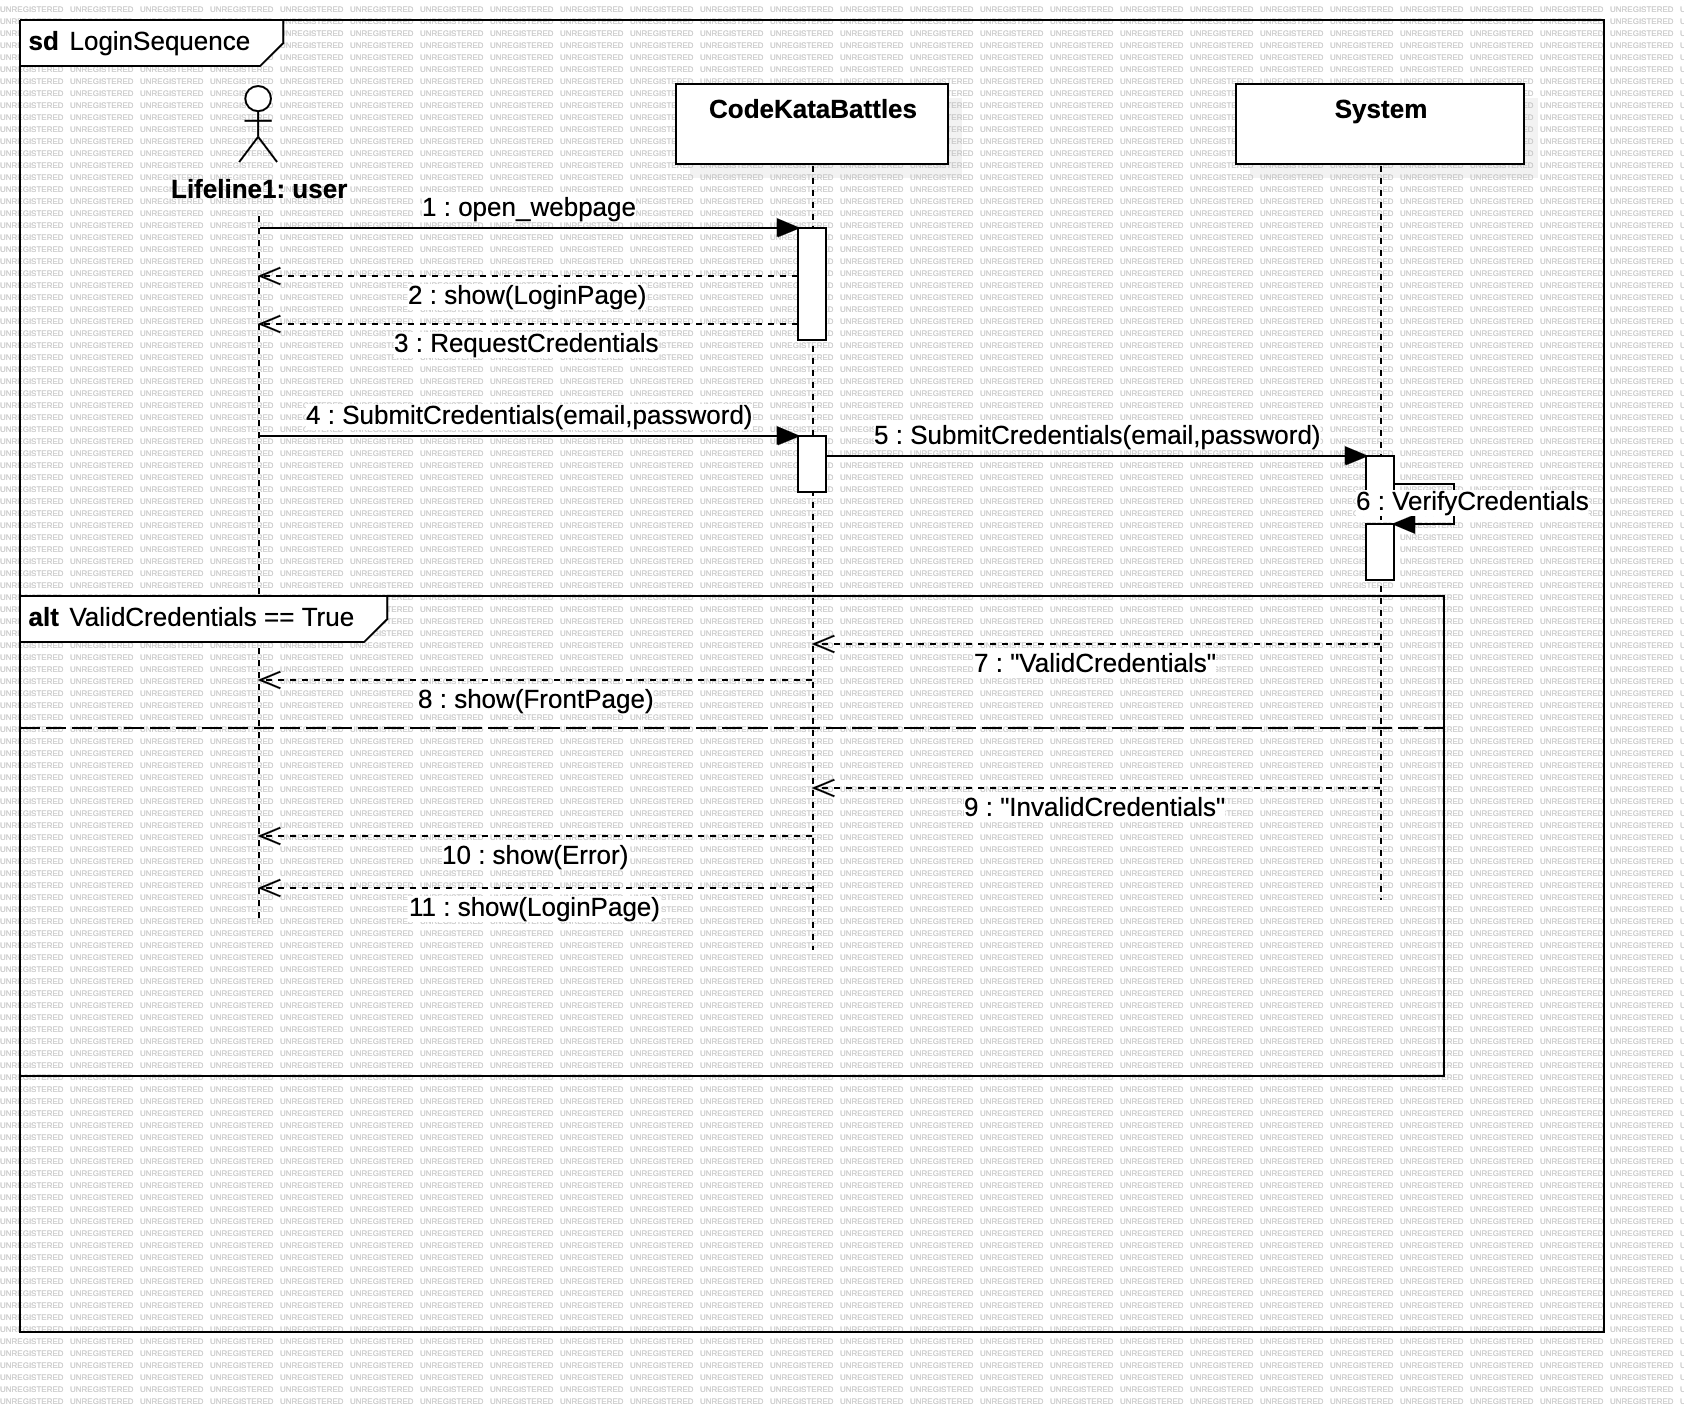
\includegraphics[width=\textwidth]{Graphics/Sequence Diagrams/LoginSequence.png}
    \caption{Sequence Diagram: Log-in Sequence}
    \label{fig:login}
\end{figure}

\newpage